\section{Experimental Setup}
\label{sec:Testbed}

Cyber-Physical Systems require design-time testing and analysis before deployment. Several CPS scenarios require strict safety certification due to the mission-critical nature of the operation, e.g. flight control and automation. It is often times impossible to test control algorithms, fault tolerance procedures etc. on the real system due to both cost and hardware accessibility issues. To counter these issues, there are two principle methods in which a CPS can be tested and analyzed: (1) Construct a complete model of the CPS in a simulation environment e.g. Simulink \cite{Simulink} and simulate the system while accounting for run-time scenarios, (2) Establish a testing environment that can closely resemble the real CPS in both hardware and software. The problem with simulations is that it is hard to establish the network topology, emulate the application network and base processing power while running a physics simulation in the loop. Our RCPS testbed implements the latter alternative. The RCPS testbed consists of 32 BBB embedded boards running Linux. The gigabit ethernet port of each BBB is connected to a programmable OpenFlow \cite{openflow} enabled \emph{Communication Network} switch. Each RCPS node is also connected to a \emph{Physics Network} using a 10/100 USB-to-Ethernet adapter, since the BBBs only have one gigabit ethernet port. This network is connected to a \emph{Physics Simulation Machine} running cyber-physical systems simulations. For further details on the architecture of this testbed, readers are referred to our earlier work \cite{kumarTestbed}.

\if 0
\begin{figure}[h]
	\centering
	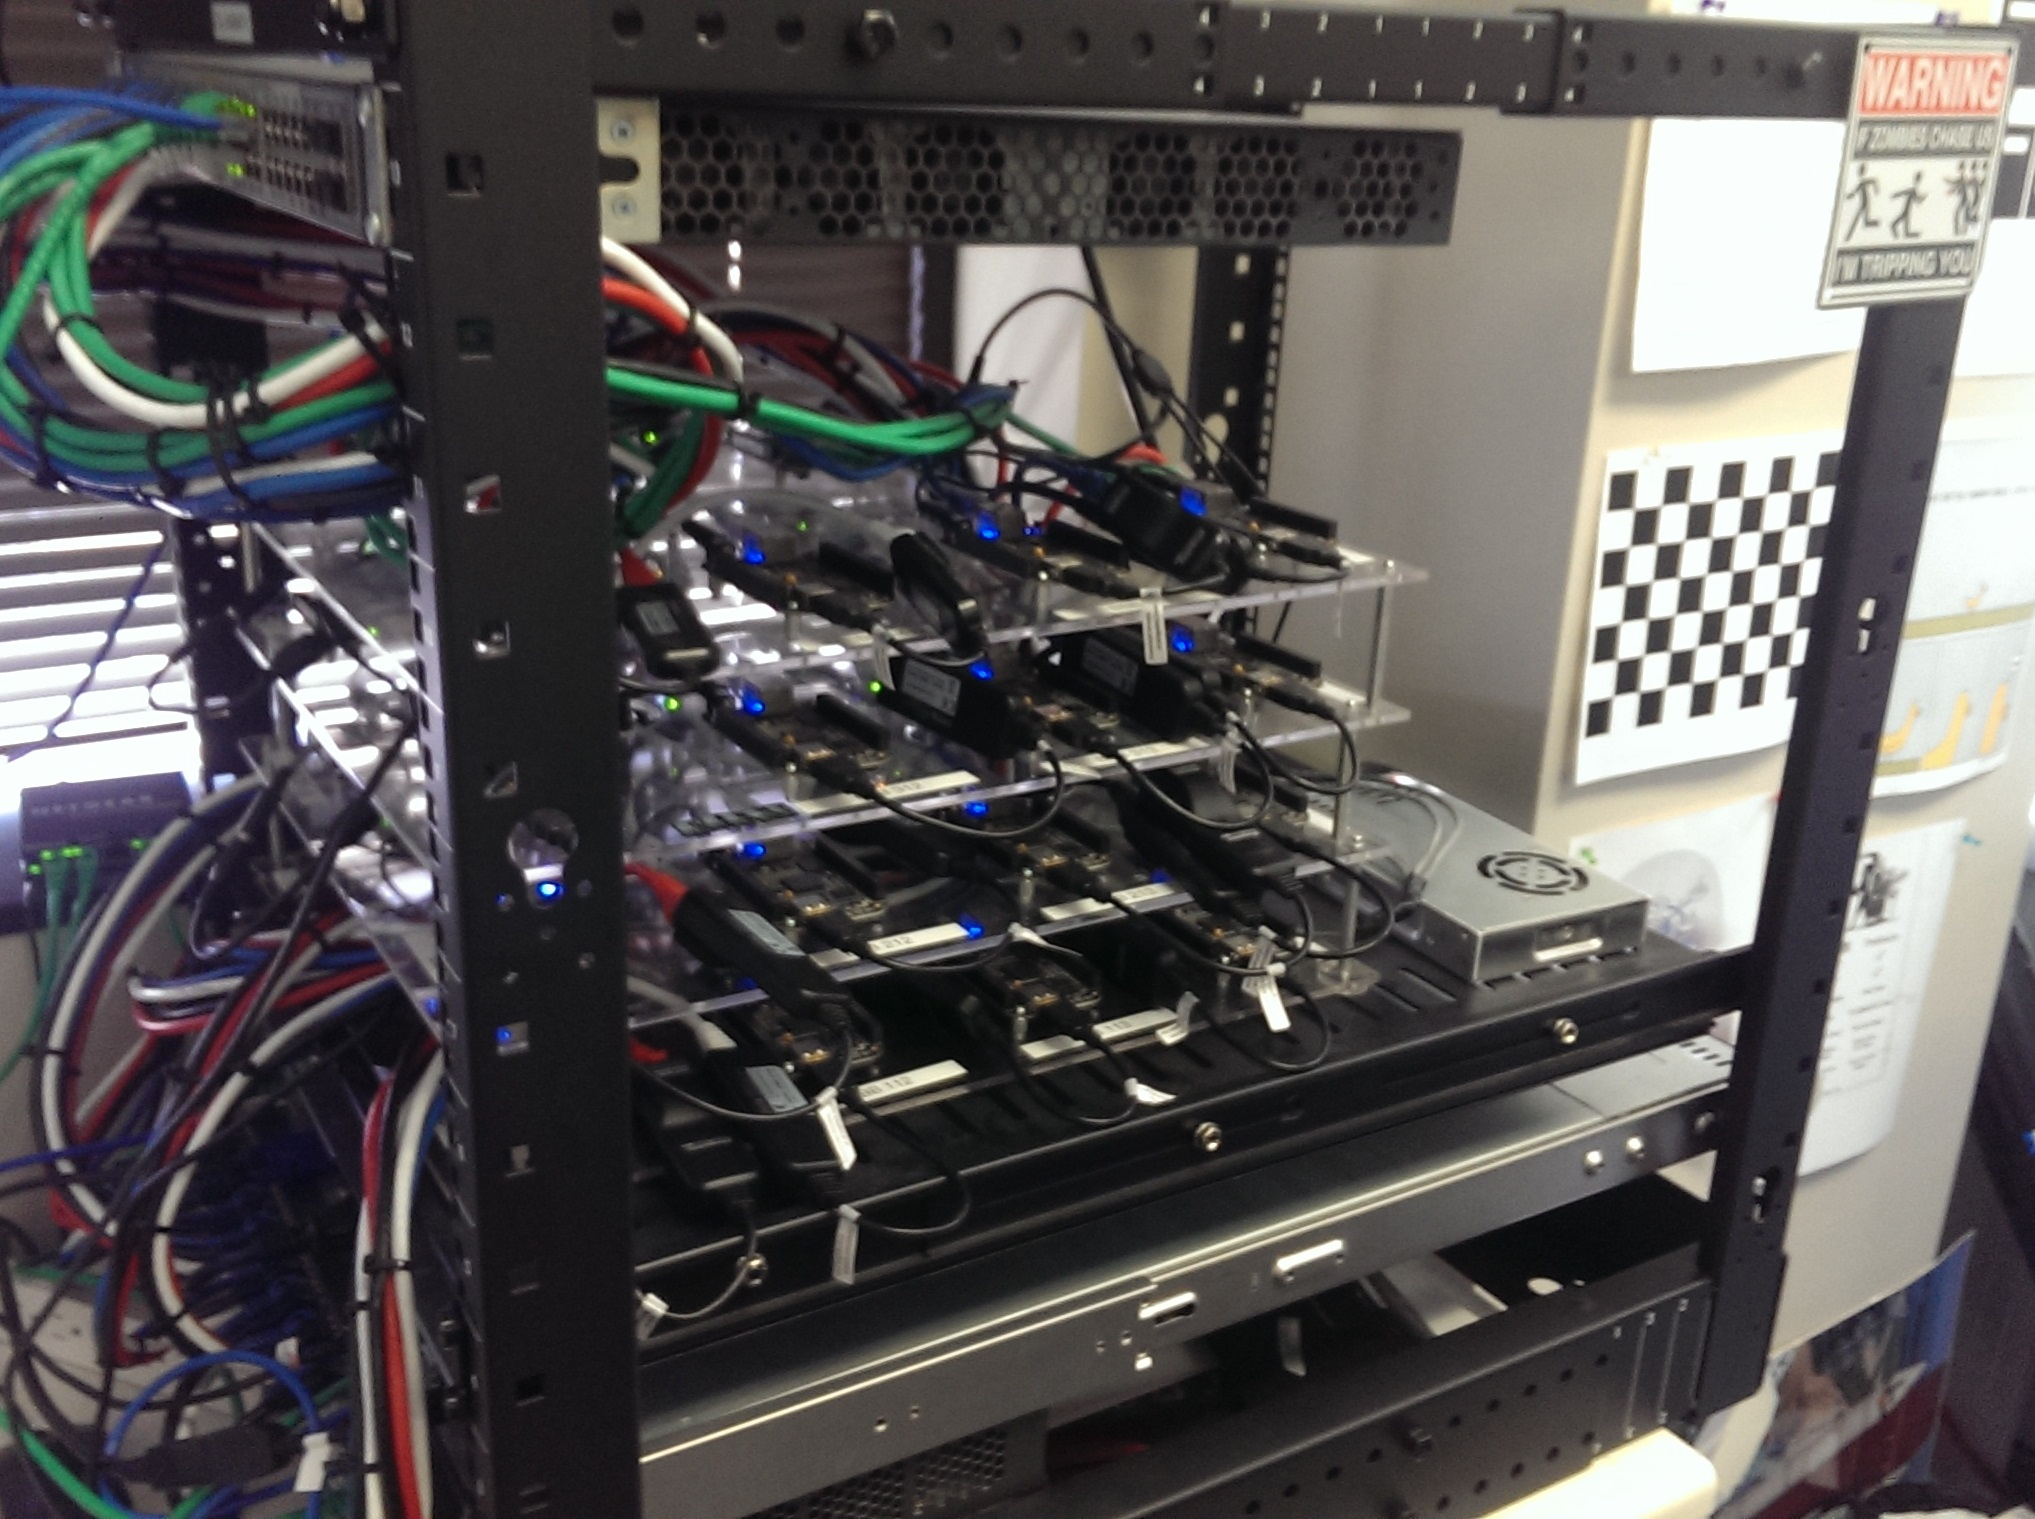
\includegraphics[width=0.45\textwidth]{testbed}
	\caption{RCPS Testbed}
	\label{fig:testbed}
\end{figure}
\fi

Using the RCPS testbed, a wide variety of DRE use-cases can be tested and accurately measured. This section briefly considers a few samples that test the various interaction patterns of ROSMOD, that are available to application developers and compares the measured results against the predicted worst-case execution time profiles of the modeled applications in our Colored Petri net-based analysis model. The expected result in all of these cases is to observe close but pessimistic behavior simulation from our analysis model i.e., the CPN analysis should be able to simulate and analyze the behaviors of the test cases and provide comparable and close approximations of the execution time plots while ensuring that the predicted \emph{worst-case execution times} (WCET), response times, processor utilization etc. are always conservative.